\documentclass[11pt, dvipsnames, handout]{beamer}
\newtoggle{full}
\settoggle{full}{true}

\newtoggle{covered}
\settoggle{covered}{false}

\newtoggle{presentable}
\settoggle{presentable}{false}

\newtoggle{dualscreen}
\settoggle{dualscreen}{false}

\usepackage{pgfplots}
%\pgfplotsset{compat = newest}

\usepackage{pgfpages}

\setbeamertemplate{note page}{\pagecolor{yellow!5}\vfill \insertnote \vfill}
\usepackage{collect}
\definecollection{notes}
\newcounter{notestaken}

\usepackage{xpatch}

\usepackage{ulem}

\usepackage[framemethod=tikz]{mdframed}

\usepackage{scalerel}
\usepackage{calc}

%\usepackage{enumitem}
\setlength\fboxsep{.2em}

\usepackage{graphicx} % Allows including images
\usepackage{booktabs} % Allows the use of \toprule, \midrule and \bottomrule in tables

\xpatchcmd{\itemize}
  {\def\makelabel}
  {\setlength{\itemsep}{0.65 em}\def\makelabel}
  {}
  {}


\xpatchcmd{\beamer@enum@}
  {\def\makelabel}
  {\setlength{\itemsep}{0.65 em}\def\makelabel}
  {}
  {}


%\makeatletter
%\renewcommand{\itemize}[1][]{%
%  \beamer@ifempty{#1}{}{\def\beamer@defaultospec{#1}}%
%  \ifnum \@itemdepth >2\relax\@toodeep\else
%    \advance\@itemdepth\@ne
%    \beamer@computepref\@itemdepth% sets \beameritemnestingprefix
%    \usebeamerfont{itemize/enumerate \beameritemnestingprefix body}%
%    \usebeamercolor[fg]{itemize/enumerate \beameritemnestingprefix body}%
%    \usebeamertemplate{itemize/enumerate \beameritemnestingprefix body begin}%
%    \list
%      {\usebeamertemplate{itemize \beameritemnestingprefix item}}
%      {%
%        \setlength\topsep{1em}%NEW
%        \setlength\partopsep{1em}%NEW
%        \setlength\itemsep{1em}%NEW
%        \def\makelabel##1{%
%          {%
%            \hss\llap{{%
%                \usebeamerfont*{itemize \beameritemnestingprefix item}%
%                \usebeamercolor[fg]{itemize \beameritemnestingprefix item}##1}}%
%          }%
%        }%
%      }
%  \fi%
%  \beamer@cramped%
%  \raggedright%
%  \beamer@firstlineitemizeunskip%
%}
%
%
%
%
%
%\makeatother

%\setlist[beamer@enum@]{topsep=1 em}
%\let\origcheckmark\checkmark %screw you dingbat
%\let\checkmark\undefined %screw you dingbat
%\usepackage{dingbat} 
%\let\checkmark\origcheckmark %screw you dingbat






%\usepackage{fontawesome}

\usepackage{mathtools}
\usepackage{etoolbox, calculator}

\usepackage{xcolor}
\usepackage{tikz}
\usetikzlibrary{arrows.meta}
\usetikzlibrary{calc}
\usepackage[nomessages]{fp}
\usepackage{transparent}
\usepackage{accsupp}
%\usepackage{color, xcolor}

%colorblind-friendly palette
%\definecolor{dblue}{RGB}{51,34,136}
\definecolor{lblue}{RGB}{136,204,238}
%\definecolor{green}{RGB}{17,119,51}
\definecolor{tan}{RGB}{221,204,119}
%\definecolor{mauve}{RGB}{204,102,119}

\usepackage{tcolorbox}



\usepackage{xifthen}
\usepackage{nicefrac}
\usepackage{amsmath}
\usepackage{amsthm}
\usepackage{amssymb}
\theoremstyle{definition}
\newtheorem*{define}{Definition}
\newtheorem*{recall}{Recall}


\DeclareMathOperator{\tr}{tr}

\usepackage{multicol}
%\setlength{\columnsep}{1cm}

\usepackage{tablists, amsmath,vwcol, cancel, polynom}
\usetikzlibrary{shapes, patterns, decorations.shapes}
%\usepackage{tikzpeople}
\tikzstyle{vertex}=[shape=circle, minimum size=2mm, inner sep=0, fill]
\tikzstyle{opendot}=[shape=circle, minimum size=2mm, inner sep=0, fill=white, draw]

% common math quick commands
\newcommand{\nicedd}[2]{\nicefrac{\text{d}#1}{\text{d}#2}}
\newcommand{\dd}[2]{\dfrac{\text{d}#1}{\text{d}#2}}
\newcommand{\pd}[2]{\dfrac{\partial #1}{\partial#2}}
\renewcommand{\d}[1]{\text{d}#1}
\newcommand{\ddn}[3]{\dfrac{\text{d}^{#3}#1}{\text{d}#2^{#3}}}
\newcommand{\pdn}[3]{\dfrac{\partial^{#3}#1}{\partial#2^{#3}}}
\newcommand{\p}[0]{^{\prime}}
\newcommand{\pp}[0]{^{\prime\prime}}
\newcommand{\op}[2][\text{L}]{#1 \left[ #2 \right]}

\newcommand{\lap}[1]{\mathcal{L}\left\{#1\right\}}
\newcommand{\lapinv}[1]{\mathcal{L}^{-1}\left\{#1\right\}}
\newcommand{\lapint}[1]{\int_0^\infty e^{-st}#1dt}
\newcommand{\evalat}[2]{\Big|_{#1}^{#2}}

\newcommand{\paren}[1]{ \left( #1 \right)}

\newcommand{\haxis}[4][\normcolor]{\draw[#1, <->] (-#2,0)--(#3,0) node[right]{$#4$}; }


\newcommand{\axis}[4]{\draw[\normcolor, <->] (-#1,0)--(#2,0) 
node[right]{$x$};
\draw[help lines, <->] (0,-#3)--(0,#4) node[above]{$y$};}

\newcommand{\laxis}[6]{\draw[<->] (-#1,0)--(#2,0) 
node[right]{$#5$};
\draw[ <->] (0,-#3)--(0,#4) node[above]{$#6$};}
\newcommand{\xcoord}[2]{
	\draw (#1,.2)--(#1,-.2) node[below]{$#2$};}
\newcommand{\textnode}[3]{
	\draw (#1,#2) node[below]{$#3$};}
	
\newcommand{\nxcoord}[2]{
	\draw (#1,-.2)--(#1,.2) node[above]{$#2$};}
\newcommand{\ycoord}[2]{
	\draw (.2,#1)--(-.2,#1) node[left]{$#2$};}
\newcommand{\nycoord}[2]{
	\draw (-.2,#1)--(.2,#1) node[right]{$#2$};}
\newcommand{\dlim}{\displaystyle\lim}
\newcommand{\dlimx}[1]{\displaystyle\lim_{x \rightarrow #1}}
\newcommand{\stickfig}[2]{
	\draw (#1,#2) arc(-90:270:2mm);
	\draw (#1,#2)--(#1,#2-.5) (#1-.25,#2-.75)--(#1,#2-.5)--(#1+.25,#2-.75) (#1-.2,#2-.2)--(#1+.2,#2-.2);}	

%\newcounter{example}
%\setcounter{example}{1}
%\newcounter{preFrameExample}
%\AtBeginEnvironment{frame}{\setcounter{preFrameExample}{\value{example}}}
%\newcommand{\ex}[1]{
%	 \setcounter{example}{\value{preFrameExample}}
%	 \textcolor{green}{\small\fbox{Example \arabic{example}: #1}}\\[8pt]
%	\stepcounter{example}}
%\newcommand{\exans}[1]{
%	\SUBTRACT{\value{preFrameExample}}{1}{\n}
%	 \textcolor{green}{\small\fbox{Solution \n: #1}}\\[8pt]}
\mode<presentation> {

% The Beamer class comes with a number of default slide themes
% which change the colors and layouts of slides. Below this is a list
% of all the themes, uncomment each in turn to see what they look like.


\usetheme{CambridgeUS}
\usecolortheme[named=black]{structure}


\newcommand{\studentcolor}[0]{ForestGreen}
\newcommand{\normcolor}[0]{NavyBlue}
\newcommand{\alertcolor}{Red}

\setbeamercolor{normal text}{fg=\normcolor}
\setbeamercolor{frametitle}{fg=\normcolor}
\setbeamercolor{section in head/foot}{fg=Black, bg=Gray!20}
\setbeamercolor{subsection in head/foot}{fg=Green!70!Black, bg=Gray!10}
\setbeamercolor{alerted text}{fg=\alertcolor}
\setbeamerfont{alerted text}{series=\bf}
\setbeamertemplate{enumerate items}[default]
\setbeamercolor{enumerate item}{fg=\normcolor}

\setbeamertemplate{footline} % To remove the footer line in all slides uncomment this line
%\setbeamertemplate{footline}[page number] % To replace the footer line in all slides with a simple slide count uncomment this line

\setbeamertemplate{navigation symbols}{} % To remove the navigation symbols from the bottom of all slides uncomment this line
}

\newcommand{\alertbox}[1]{\tcbox[on line, colframe=\alertcolor, colback=White, left=2pt,right=2pt,top=2pt,bottom=2pt]{\usebeamercolor*{normal text}#1}}


\newcommand{\startstu}{\setbeamercolor{normal text}{fg=\studentcolor}\usebeamercolor*{normal text}\setbeamercolor{enumerate item}{fg=\studentcolor}\usebeamercolor*{enumerate item}}
\newcommand{\stopstu}{\setbeamercolor{normal text}{fg=\normcolor}\usebeamercolor*{normal text}\setbeamercolor{enumerate item}{fg=\normcolor}\usebeamercolor*{enumerate item}}

\newcommand{\takenote}[1]{ \begin{collect}{notes}{}{}{}{}  #1  \end{collect}  \addtocounter{notestaken}{1}} %\ifthenelse{\value{notestaken}>0}{\hrulefill\\}{}

\makeatletter
\newcommand{\cover}{\alt{\beamer@makecovered}{\beamer@fakeinvisible}}
\newcommand{\ucover}[1]{\iftoggle{full}{}{\beamer@endcovered}\stopstu#1\startstu\iftoggle{full}{}{\beamer@startcovered}}
\makeatother

\newcommand{\skippause}{ \addtocounter{beamerpauses}{-1}}
\newcommand{\blockpres}{ \skippause \pause }

\newcommand{\studentify}[1]{\startstu #1  \stopstu }
\newcommand{\student}[1]{\iftoggle{full}{ \pause  \studentify{#1} }{\iftoggle{covered}{\studentify{#1}}{\cover{  #1 }}}}
\newcommand{\cstudent}[1]{\student{\begin{center} #1 \end{center}}}
\newcommand{\fullonly}[1]{\iftoggle{full}{ #1}{}}
\newcommand{\presentonly}[1]{\iftoggle{presentable}{ #1}{}}

\usepackage{xparse}
\usepackage{xifthen}

% shortcuts for commonly-used presentation elements
%\NewDocumentCommand{\slide}{o m}
% {\IfValueTF{#1}{\begin{frame}[t]{#1}}{\begin{frame}[t]} #2 \end{frame}}

\newtoggle{iscovered}

\newcommand{\slide}[2][]{%
%\setcounter{notestaken}{0}
\takenote{#2} 
%\ifthenelse{\equal{#1}{}}{\begin{frame}[t]}{\begin{frame}[t]{#1}} #2 \ifthenelse{\value{notestaken}>0}{ \note{\includecollection{notes}}}{} \end{frame}%
\ifthenelse{\equal{#1}{}}{\begin{frame}[t]}{\begin{frame}[t]{#1}} #2 \iftoggle{covered}{\settoggle{iscovered}{true}}{\settoggle{iscovered}{false}}  \note{ \iftoggle{iscovered}{}{\settoggle{covered}{true}} #2 \iftoggle{iscovered}{}{\settoggle{covered}{false}} } \end{frame}%
%\setcounter{notestaken}{0}
}
\newcommand{\defn}[2][]{%
 \setcounter{listcounter}{0}%
\ifthenelse{\equal{#1}{}}{\begin{block}{Definition}}{\begin{block}{#1 :}}%
 #2 \vspace{0.25em} \ifthenelse{\value{listcounter}>0}{\skippause}{} \pause \end{block}%
}



\newcommand{\arr}[2]{\begin{array}{#1}#2\end{array}}
\newcommand{\mat}[2]{\left[\arr{#1}{#2}\right]}
\newcommand{\carray}[1]{\arr{c}{#1}}
\newcommand{\larray}[1]{\arr{l}{#1}}
\newcommand{\rarray}[1]{\arr{r}{#1}}
\newcommand{\colvec}[1]{\mat{c}{#1}}

\newcommand{\itmz}[1]{\addtocounter{listcounter}{1} \begin{itemize}#1 \end{itemize} }
\newcommand{\subitem}[1]{\addtocounter{listcounter}{1} \begin{itemize} \item #1 \end{itemize}}
%
\newcommand{\enum}[1]{\addtocounter{listcounter}{1} \begin{enumerate} #1  \end{enumerate}  }


\newcommand{\algnlbl}[1]{\begin{align}#1  \end{align}} 
\newcommand{\algn}[1]{\begin{align*}#1  \end{align*}} 
\newcommand{\lgn}[1]{ \action<+->{#1} }
\newcommand{\slgn}[1]{\iftoggle{full}{\action<+->{ \startstu #1 \stopstu}}{ \cover{ #1 } } \takenote{$#1$}}

\newcommand{\chckmrk}{\alert{\checkmark}}

\usepackage{pifont}
\newcommand{\xmark}{\alert{\text{\large \ding{55}}}}

\newcommand{\return}[0]{\raisebox{.5ex}{\rotatebox[origin=c]{180}{$\Lsh$}}}
\usepackage{pbox}
%\newcommand{\ex}[1]{\rotatebox[origin=c]{10}{\uline{ex}}:$\;$\pbox[t][][b]{0.9\linewidth}{#1}}
\newcommand{\ex}[1]{\uline{ex}:$\;$\pbox[t][][t]{0.9\linewidth}{#1}}
\newcommand{\eg}[1]{e.g.,$\;$\pbox[t][][t]{0.9\linewidth}{#1}}
\newcommand{\tikzplot}[8][]{%
\begin{tikzpicture}

\begin{scope}[]%
\clip(-#2,-#4) rectangle (#3,#5);%
#8%
\end{scope}%
\laxis{#2}{#3}{#4}{#5}{#6}{#7}%
#1
\end{tikzpicture}%
}


\newcommand{\cancelslide}[1]{%
\begingroup%
\setbeamertemplate{background canvas}{%
\begin{tikzpicture}[remember picture,overlay]%
\draw[line width=2pt,red!60!black] %
  (current page.north west) -- (current page.south east);%
\draw[line width=2pt,red!60!black] %
  (current page.south west) -- (current page.north east);%
\end{tikzpicture}}%
#1%
\endgroup%
}
\renewcommand{\CancelColor}{\color{red}}
\newcommand{\twocols}[3][0.5]{\begin{columns}\begin{column}{#1\textwidth}#2\end{column}\hspace{1em}\vrule{}\hspace{1em}\begin{column}{#1\textwidth}#3\end{column}\end{columns}}

\newcommand{\twomini}[5][1]{\calculatespace \begin{minipage}[t]{\columnwidth}\begin{minipage}[][#1\contentheight][t]{#2\columnwidth}#4\end{minipage}\hfill\begin{minipage}[][#1\contentheight][t]{#3\columnwidth}#5\end{minipage}\end{minipage}}

\newcommand{\threemini}[7][1]{\calculatespace \begin{minipage}[t]{\columnwidth}\begin{minipage}[][#1\contentheight][t]{#2\columnwidth}#5\end{minipage}\hfill\begin{minipage}[][#1\contentheight][t]{#4\columnwidth}#6\end{minipage}\hfill\begin{minipage}[][#1\contentheight][t]{#3\columnwidth}#7\end{minipage}\end{minipage}}


\newcounter{listcounter}
\setcounter{listcounter}{0}



\newif\ifsidebartheme
\sidebarthemetrue

\newdimen\contentheight
\newdimen\contentwidth
\newdimen\contentleft
\newdimen\contentbottom
\makeatletter
\newcommand*{\calculatespace}{%
\contentheight=\paperheight%
\ifx\beamer@frametitle\@empty%
    \setbox\@tempboxa=\box\voidb@x%
  \else%
    \setbox\@tempboxa=\vbox{%
      \vbox{}%
      {\parskip0pt\usebeamertemplate***{frametitle}}%
    }%
    \ifsidebartheme%
      \advance\contentheight by-1em%
    \fi%
  \fi%
\advance\contentheight by-\ht\@tempboxa%
\advance\contentheight by-\dp\@tempboxa%
\advance\contentheight by-\beamer@frametopskip%
\ifbeamer@plainframe%
\contentbottom=0pt%
\else%
\advance\contentheight by-\headheight%
\advance\contentheight by\headdp%
\advance\contentheight by-\footheight%
\advance\contentheight by4pt%
\contentbottom=\footheight%
\advance\contentbottom by-4pt%
\fi%
\contentwidth=\paperwidth%
\ifbeamer@plainframe%
\contentleft=0pt%
\else%
\advance\contentwidth by-\beamer@rightsidebar%
\advance\contentwidth by-\beamer@leftsidebar\relax%
\contentleft=\beamer@leftsidebar%
\fi%
}
\makeatother



\iftoggle{dualscreen}{\setbeameroption{show notes on second screen=right}}{}
\usetikzlibrary{arrows}
\usetikzlibrary{decorations.markings}
\settoggle{covered}{true}
\begin{document}
\section{Lecture 26}
\subsection{Preamble}
\slide[Introduction]{

Almost all nonlinear systems cannot be solved analytically. Instead, we can use local stability analysis to gain qualitative infomation about solutions.
\vfill
\enum{\item ~ \student{Classify the stability and type of all fixed points\subitem{Fixed points can lose stability, collide, and/or dissapear/appear as system parameters are changed.}}\vfill

\item ~\student{Draw phase plane sketches to get a geometric picture \subitem{Use the fact that derivatives switch sign when trajectories cross nullclines}}}
\vfill
}


\subsection{Lamps vs. Lasers}
\slide[Lamps]{
Lamps work at a quantum level  by pumping  molecules into an excited state, such that they release photons (light particles) as they return back down to the ground state.\vfill
\twomini[.5]{.5}{.5}{
\centerline{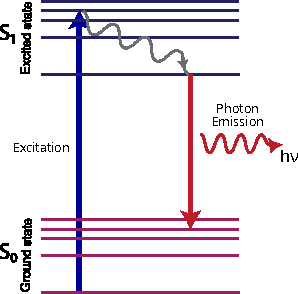
\includegraphics[width=.7\columnwidth]{images/Jablonski_lamp.pdf}}
}{
\vspace{3em}
\centerline{
\includegraphics[width=.8\columnwidth]{images/incoherent.png}}
}\vfill
The excitation/emission process is random, producing photons with uncorrelated phases and orientation. This is what we call \uline{incoherent} light.
}

\slide[Lasers \hfill \small (\textbf{L}ight \textbf{A}mplification by \textbf{S}timulated \textbf{E}mission of \textbf{R}adiation)]{\vspace{-1em}
Lasers work through a process called \textbf{stimulated emission}, photon emission from one molecule triggers the emission of a photon by its neighbour with \uline{similar phase and orientation}.\vspace{1.5em}
\twomini[.5]{.65}{.35}{
\centerline{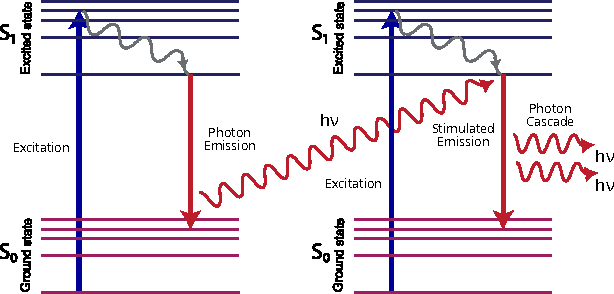
\includegraphics[width=\columnwidth]{images/Jablonski_laser.pdf}}
}{
\vspace{3em}
\centerline{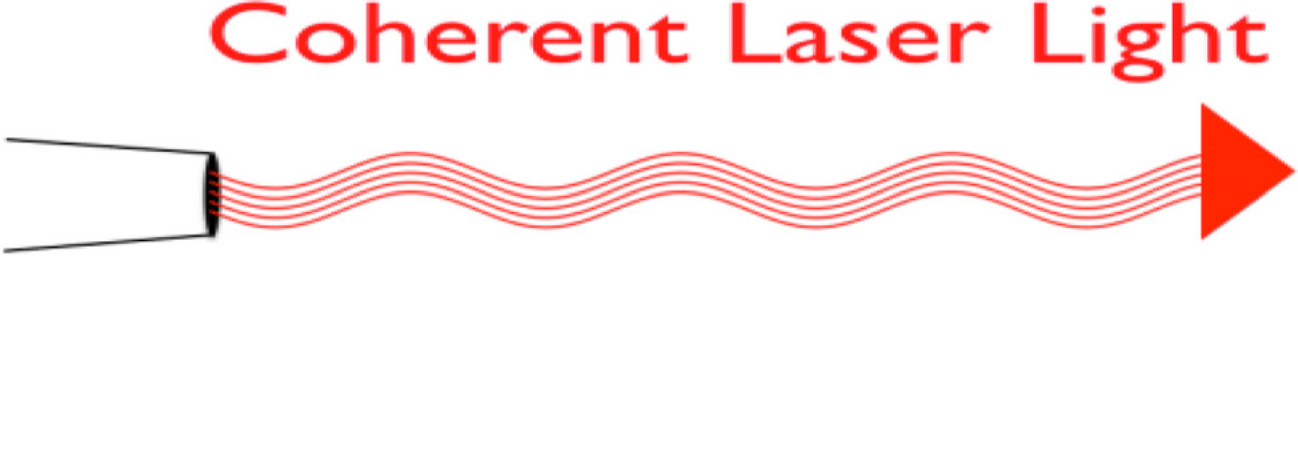
\includegraphics[width=.9\columnwidth]{images/coherent.png}}
}\vspace{1.5em}


If enough stimulated emission happens, we get an emission cascade of photons with highly correlated phase and orientation. This results in \uline{coherent} light beams that can travel long distances with minimal spread.
}

\subsection{Lamps vs. Lasers}
\slide{
A simple model for a laser considers two variables: \enum{\item $N(t)$ = \student{\# of ``ordinary'' excited molecules }\item $n(t)$ = \student{\# of ``lasing'' molecules that will emit photons coherently.}}
\vfill
The dynamics of the two variables are given by 
\vspace{.5em}
\student{\algn{n' &= nN-n\\ N' &= -nN-N+p}}
\vspace{.5em}

where $p$ is a ``pumping'' parameter that quantifies the rate of excitation.
\vfill
see Laser Physics by  Miloni and Eberly (1988) for more details.
}

\slide{
\ex{Find all critical points for the system: }
\[ n' = nN-n,\quad N' = -nN-N+p \]
\vfill
\student{
\algn{\text{\uline{n-nullclines:}}& & \text{\uline{N-nullclines:}}&\\
0&=n(N-1) &0&=-N(1+n)+p\\
n=0&\quad \text{and}\quad  N=1 &N&=\frac{p}{1+n}\intertext{intersections}
n=0\;\; \&\;\; N&=\frac{p}{1+n}\Rightarrow N=p\\
N=1\;\; \& \;\; N&=\frac{p}{1+n}\Rightarrow  n =p-1\\
&\qquad \qquad \Rightarrow N=1
}
\vfill
\[\uline{\text{critical points:}} \quad \underbrace{(0,p)}_{\text{lamp}}, \quad \text{and} \quad \underbrace{(p-1, 1)}_{\text{laser}}\]
}
}




\slide{\vspace{-.5em}
\ex{Given the simple laser model}
\[ n' = nN-n,\quad N' = -nN-N+p, \]
find a condition on $p$ that ensures that the laser state is the unique stable steady state.\vspace{-0.5em}
\student{
\[\mathbf{J} = \mat{cc}{N-1 & n \\ -N & -n-1}\]
\vspace{-2.5em}

\algn{
\text{\uline{lamp:}}& \quad (0,p) & \text{\uline{laser:}}& \quad (p-1,1)\\
\mathbf{J}^* &= \mat{cc}{p-1 & 0 \\ -p & -1} & \mathbf{J}^* &= \mat{cc}{0 & p-1 \\ 1 & -p}
\intertext{Find the eigenvalues, i.e., $\det({J}^*-\lambda \mathbf{I}) =0$ }
(p-1-\lambda)(-1-\lambda)&=0 & -\lambda(-p-\lambda)&+1-p=0\\
\lambda&=p-1, -1 &\lambda^2-p\lambda+1-p&=0\\
&&\lambda = \frac{-p}2 \pm & \frac{\sqrt{(p-2)^2}}{2}&\\
&&=-1,1&-p
}
}
}

\slide{\vspace{-.5em}
\ex{Given the simple laser model}
\[ n' = nN-n,\quad N' = -nN-N+p, \]
find a condition on $p$ that ensures that the laser state is the unique stable steady state.\vspace{-0.5em}


\algn{
\text{\uline{lamp:}}& \quad (0,p) & \text{\uline{laser:}}& \quad (p-1,1)\\
\lambda &= p-1, -1 &\lambda &= -1,1-p
}
\vfill
\student{

Both steady states have an eigenvalue of -1, independent of $p$.
\vfill
For $p<1$, the lamp state is a stable  node and the laser state is a saddle (unstable).
\vfill
For $p>1$, the lamp state is a saddle and the laser state is stable node.

}
}

\slide[Laser Threshold]{
The laser and lamp steady states collide at $p=1$ and exchange their stability.
\centerline{
\tikzplot[\xcoord{2}{1}]{.1}{6}{1}{4}{p}{n^*}{
\draw[ultra thick, black] (0,0) -- (2,0);\draw[ultra thick, black, dashed] (2,0) -- (6,0);
\draw[Black] (1.25,.25) node{lamp};
\draw[ultra thick, black] (2,0) -- (6,2);\draw[ultra thick, black, dashed] (0,-1) -- (2,0);
\draw[Black] (4,1.5) node{laser};
\draw[black,->] (5,0.5)--(5,1.25);\draw[black,->] (5,2.5)--(5,1.75);
\draw[black,->] (.5,.75)--(.5,.25);\draw[black,->] (.5,-.65)--(.5,-.25);
}
}

}

\settoggle{covered}{false}

\subsection{Phase Plane Analysis of Limit Cycles}

\slide[Your heart beats cyclically]{\vspace{-1em}
The Sinoatrial (SA) node is the main clock.
\vfill
\twomini[.56]{0.475}{0.475}{
\centerline{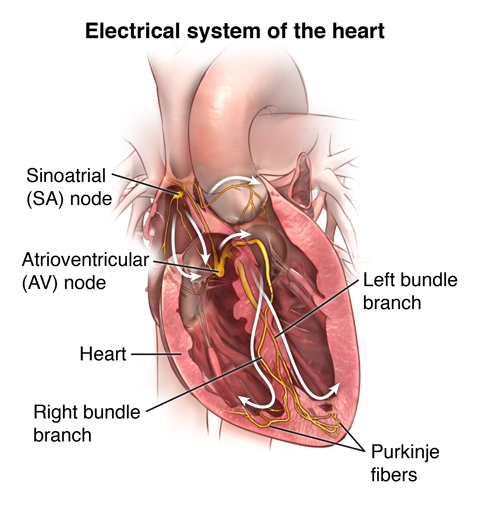
\includegraphics[width=.55\columnwidth]{images/heart electrical system.png}}
\tiny source: https://www.hopkinsmedicine.org/health/conditions-and-diseases/anatomy-and-function-of-the-hearts-electrical-system

}{
\centerline{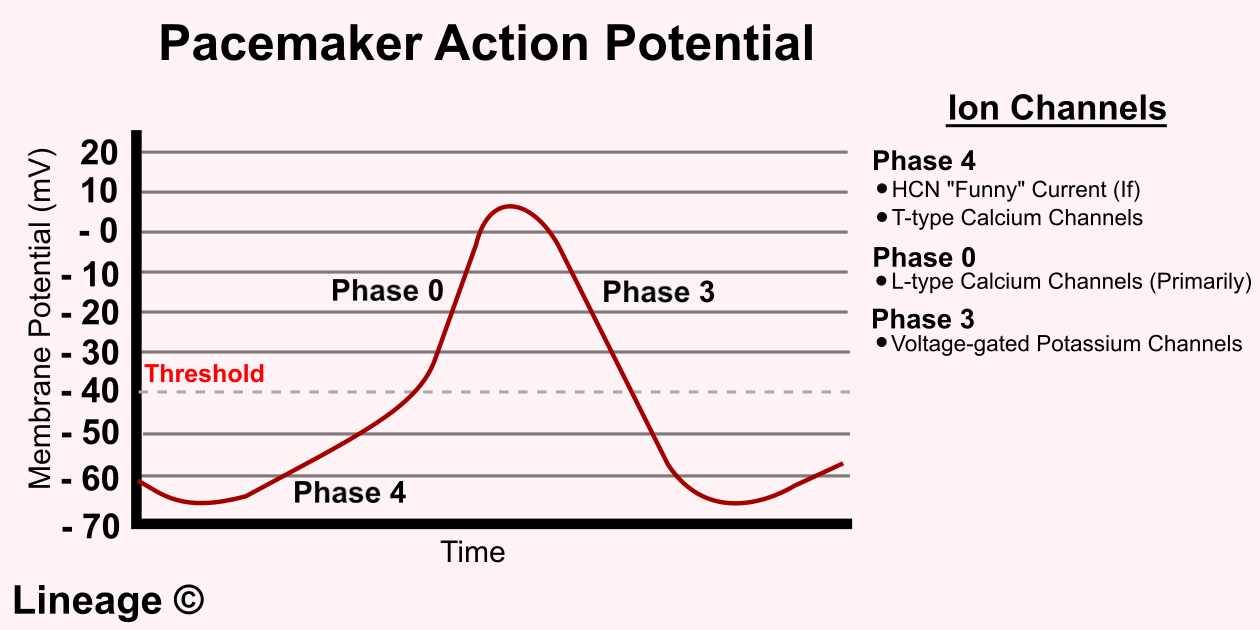
\includegraphics[width=\columnwidth]{images/pacemaker ap.jpg
}}
\tiny source: https://step1.medbullets.com/cardiovascular/108016/sa-node-action-potential

}
\vfill
\centerline{ These oscillations must be robust to perturbations, otherwise you would die :( }


\vfill
\student{Such periodic solutions are called stable limit cycles \subitem{ i.e., a cycle (or closed loop) that the nonlinear system approaches in the limit $t\to \infty$ }}
}


\slide[Limit Cycles]{
A limit cycle is an isolated closed trajectory. Isolated means that neighboring trajectories are not closed; they spiral either toward or away from the limit cycle.
\vfill
\student{\centerline{Spiral trajectories $\Rightarrow$ complex conjugate eignevalues.}}
\vfill
\centerline{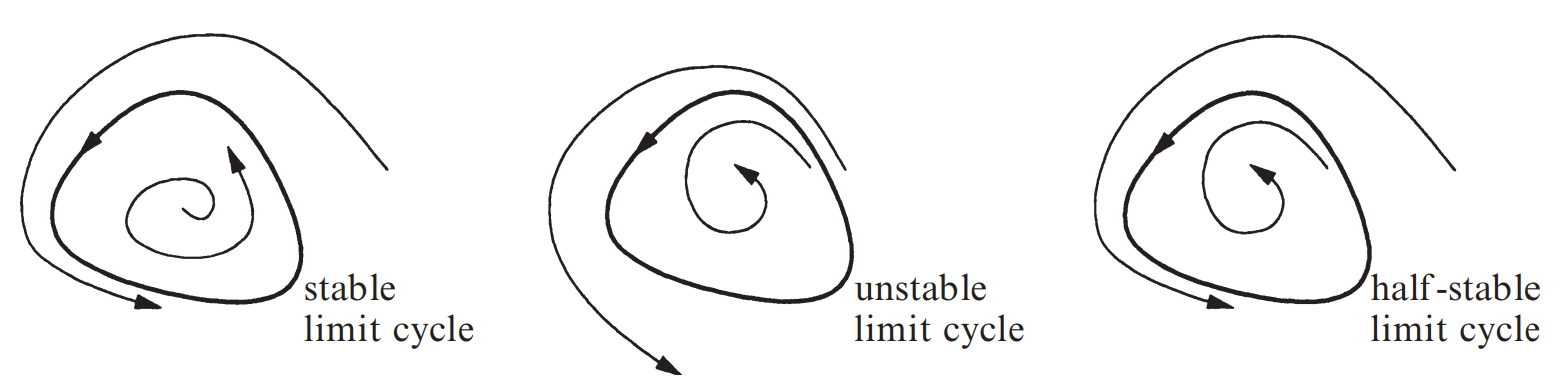
\includegraphics[width=0.8\columnwidth]{images/limit_cycles.png}}
\vfill
\student{\centerline{Stable limit cycles form around unstable spiral fixed points}}
}

\slide[Van der Pol Oscillator]{

The Van der Pol Oscillator is a simple model that exhibits limit cycles. Its dynamics are given by \student{\[x'  = y - \frac13 x^3+x,\quad y'=a-x  \]} where $a$ is a forcing parameter.
\vfill
Find the nullclines for this model.
\student{
\algn{\text{\uline{x-nullcline:}}& & \text{\uline{y-nullcline:}}&\\
y&=\frac13 x^3-x & x&=a}
}

}
\slide[Van der Pol Oscillator]{
The Van der Pol Oscillator has a \uline{unique} fixed point at
\student{\[x=a, \quad  y = \frac13 a ( a^2-3) \]}
with eigenvalues given by
\student{\[\lambda = \frac12 \left(1 - a^2 \pm \sqrt{ a^4 - 2 a^2-3}\right) .\]

These are complex conjugate eigenvalues that become stable for $|a|>1$.
\vfill
Unstable spiral for $|a|<1$.
\vfill
Stable spiral for $|a|>1$.

}
}

\slide{
Use the nullclines to sketch a solution trajectory for \[x'  = y - \frac13 x^3+x,\quad y'=a-x  \] with a=-1.5 starting at (0,-0.5)


\centerline{
\tikzplot[\xcoord{2}{1}\xcoord{-2}{-1}\ycoord{2}{1}\ycoord{-2}{-1}]{5}{5}{2.5}{2.5}{x}{y}{
\draw[ultra thick, domain=-2.5:2.5, smooth] plot ({2*\x},{2*\x*\x*\x/3-2*\x}) ;
\draw[] (3,2) node{x-nullcline};
\draw[ultra thick, dashed] (-3,-3)--(-3,3);
\draw[] (-1.95,-1.5) node{y-nullcline};
\filldraw[] (-3,0.75) circle (3pt);
\draw[] (0,-1) node[opendot]{};
\student{
\draw(1.5,-2) node[align=center]{$x'<0$\\$y'<0$};
\draw(-3.6,-2) node[align=center]{$x'<0$\\$y'>0$};
\draw(-4,1.5) node[align=center]{$x'>0$\\$y'>0$};
\draw(-1,2) node[align=center]{$x'>0$\\$y'<0$};
}
}
}

}




\slide{
Use the nullclines to sketch a solution trajectory for \[x'  = y - \frac13 x^3+x,\quad y'=a-x  \] with a=0.5 starting at (0,-0.25)


\centerline{
\tikzplot[\xcoord{2}{1}\xcoord{-2}{-1}\ycoord{2}{1}\ycoord{-2}{-1}]{5}{5}{2.5}{2.5}{x}{y}{
\draw[ultra thick, , domain=-2.5:2.5, smooth] plot ({2*\x},{2*\x*\x*\x/3-2*\x}) ;
\draw[] (3.2,2) node{x-nullcline};
\draw[ultra thick, dashed, ] (1,-3)--(1,3);
\draw[] (1.95,-2.3) node{y-nullcline};
\filldraw[] (1,-0.916667) circle (3pt);
\draw[] (0,-0.5) node[opendot]{};

\node[rectangle, draw ,align=center] (r) at (-2,-1.8)  {$x'<0$\\$y'>0$};
\node[rectangle, draw ,align=center] (r) at (3.6,-1.8) {$x'<0$\\$y'<0$};
\node[rectangle, draw ,align=center] (r) at (-4,1.5) {$x'>0$\\$y'>0$};
\node[rectangle, draw ,align=center] (r) at (2.5,1){$x'>0$\\$y'<0$};

}
}\vfill
Note: the solution trajectory should approach a stable limit cycle
}



\end{document}
